\section{Le contexte}
\paragraph{}
Au moment de travailler sur ce projet, j'ai passé 5 semestres comme étudiant à la Faculté d'Informatique, Iași, et le dernier (en cours) comme étudiant \href{https://ec.europa.eu/programmes/erasmus-plus/about_en}{Erasmus}, à l'Université de Lille.
Comme le destin l'a voulu, l'épidémie de \href{https://en.wikipedia.org/wiki/2019-20_coronavirus_pandemic-20_coronavirus_pandémique}{COVID-19} nous force actuellement à nous isoler pendant au moins deux semaines, alors quelle meilleure occasion de passer du temps de qualité à travailler sur ce projet?
% At the time of working on this project, I've spent 5 semesters as a student at Faculty of Computer Science, Iași, and the last (current) one as an \href{https://ec.europa.eu/programmes/erasmus-plus/about_en}{Erasmus} student, at Université de Lille.
% As fate has it, the \href{https://en.wikipedia.org/wiki/2019–20_coronavirus_pandemic}{COVID-19} outbreak is currently forcing us into at least 2 weeks of self-isolation, so what better opportunity to spend quality time working on this?
\paragraph{}
Il s'agit d'un projet à double objectif.
En tant qu'étudiant Erasmus, j'aurai développé ce projet pour le cours \href{https://www.fil.univ-lille1.fr/portail/index.php?dipl=MInfo&sem=S8&ue=PJI&label=Présentation}{``Projet Individuel''}, ayant un soutenance finale à la fin du mois de Mai, 2020.
Après avoir terminé le programme Erasmus, le projet aura servi de thèse pour l'obtention d'une Licence, à la Faculté d'Informatique, Iași.
% This is a double purposed project.
% As an Erasmus student, I will have developed this project for the \href{https://www.fil.univ-lille1.fr/portail/index.php?dipl=MInfo&sem=S8&ue=PJI&label=Présentation}{``Projet Individuel'' course}, having a final soutenance at the end of May, 2020.
% After having finished the Erasmus programme, the project will have been used as my thesis to obtain a Bachelor's Degree, at Faculty of Computer Science, Iași.

\section{L'idée}
\paragraph{}
L'idée de base est d'avoir une logiciel qui suivra le visage de l'utilisateur, avec le but de déplacer la position du curseur en temps réel.
Pour cela, nous utiliserons une webcam pour obtenir des images.
Avec ceux, nous essaierons de calculer l'endroit où l'utilisateur regarde et de déplacer le curseur de la souris en conséquence.
% The base idea is to have a software application that will track the user's face, with the purpose of moving the cursor position in real time.
% For this, we will make use of a webcam to get image input.
% Further, based on the image, we will try to calculate where the user is looking and finally move the mouse cursor accordingly.
\begin{figure}[H]
    \centering
    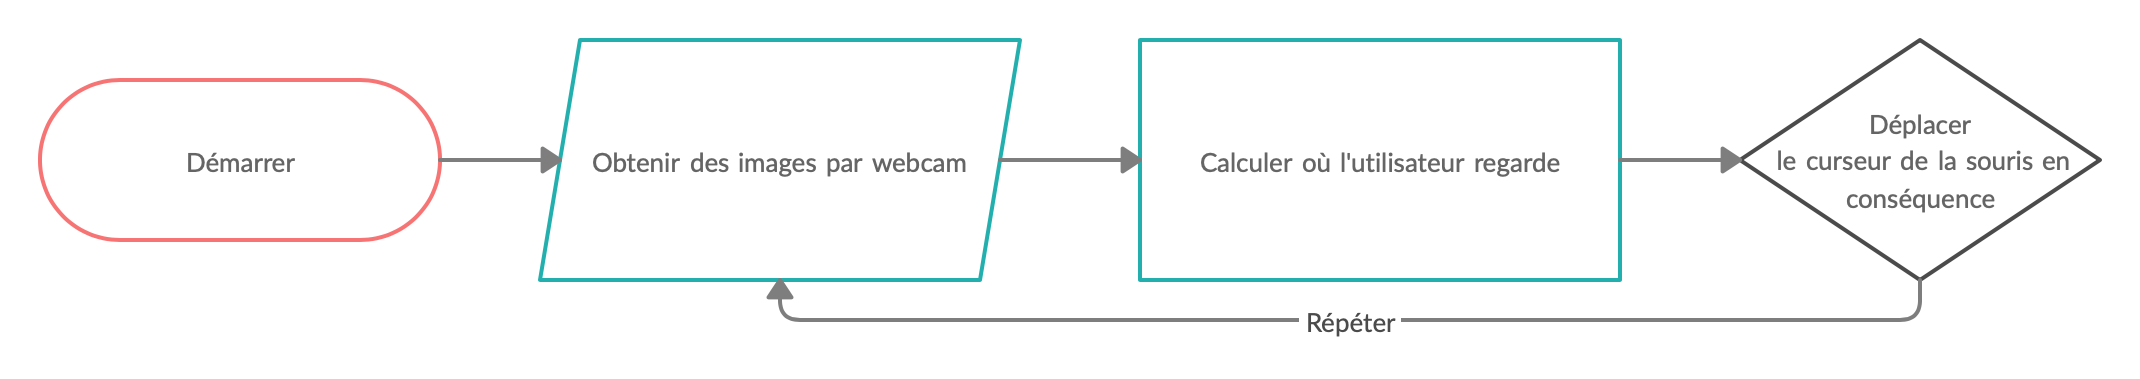
\includegraphics[width=\textwidth]{app_idea.png}
    \caption{Procédure générale}
\end{figure}

\section{Motivation}
\paragraph{}
Pour décider le projet sur lequel je voulais travailler, j'ai pris en compte deux facteurs clés: ma future carrière professionnelle et la facilité d'utilisation du projet.
Je voulais travailler sur un projet qui alimenterait mon intérêt pour l'Intelligence Artificielle et qui me donnerait la possibilité d'appliquer les recherches que je ferai dans ce domaine.
Aussi, je voulais avoir une approche pratique de ce projet et faire quelque chose qui soit utile aux gens.
% When it came to deciding what project I wanted to work on, I took into account 2 key factors: my future professional career and the project's usability.
% I wanted to work on something that would fuel my interest in Artificial Intelligence and that would give me a chance to apply the research I will be making into this field.
% Furthermore, I also wanted to have a practical approach towards this project and make something that will be useful for people.
\paragraph{}
Si l'on regarde en arrière, on constate que les gens ont toujours travaillé à rendre la technologie accessible au plus grand nombre.
Qu'il s'agisse du système braille, de l'aide aux aveugles pour lire et écrire, des lecteurs d'écran ou des assistants intelligents (Siri, Bixby, etc.), l'accessibilité est un facteur clé pour faire en sorte que les gens bénéficient des avantages de la technologie.
Par conséquent, je serais rassuré de savoir que j'ai moi aussi travaillé sur un projet qui pourrait potentiellement aider les personnes handicapées – et pas seulement elles – à utiliser l'ordinateur sans l'aide des mains.
% Looking back in time, people have always worked on making technology accessible to as many people as possible.
% Whether we're talking about the Braille system, helping blind people read and write, screen readers or intelligent assistants (Siri, Bixby etc.), accessibility is a key factor in making sure that people benefit from the advantages of technology.
% Therefore, I'd feel a certain peace of mind knowing that I too worked on a project that could potentially help disabled people – and not only them – use the computer without the use of hands.
\paragraph{}
Quant à l'Intelligence Artificielle, il est inutile de souligner son importance contemporaine.
De l'applicabilité médicale, de la conduite et du pilotage autonomes et l'agriculture intelligente aux réfrigérateurs intelligents qui vous disent quand vous êtes à court de lait, l'Intelligence Artificielle est très répandue et sa croissance ne va pas s'arrêter de sitôt.
Pour moi, c'est une raison supplémentaire de l'étudier et de mieux la comprendre, car elle est intégrée dans notre vie quotidienne.
% As for Artificial Intelligence, it is needless to emphasize it's contemporany importance.
% From medical applicability, autonomous driving and flying, smart agriculture to having smart fridges that tell you when you're running out of milk, Artificial Intelligence is widespread and it's growth isn't going to stop anytime soon.
% For me, this is another reason to study it and get to understand it better, since it is being integrated in our everyday lives.
% % As a bonus, I'll have the chance of using some of the knowledge I've gathered as a student throughout the time.
% % to individually work on a project that will showcase my software development skills, but also the abilities of practical knowledge applying and researching on certain topics.

\section{Le but}
\subsection{Objectifs essentiels}
\paragraph{}
\label{chapter-introduction-first-objective}
L'un des premiers objectifs que j'essaierai d'atteindre est de savoir approximativement où l'utilisateur regarde en utilisant uniquement ses yeux.
Par exemple, un bon début serait de savoir sur quelle partie de l'écran l'utilisateur se concentre.
En se basant sur la grille ci-dessous, si l'utilisateur regarde le carré numéro $i$, alors nous déplacerons le curseur de la souris au centre de ce carré.
Je vais expérimenter avec différentes tailles de grille, comme 2x2, 3x3 et 4x4.

% One of the first objectives I'll try to meet is approximately knowing where the user is looking only using the user's eyes.
% For example, a good start would be to know which portion of the screen the user is focusing on.
% Based on the grid below, if the user looks at square number $i$, then we will move the mouse cursor in the center of that square.
% I will experiment with different grid sizes, like 2x2, 3x3 and 4x4
\begin{figure}[H]
    \centering
    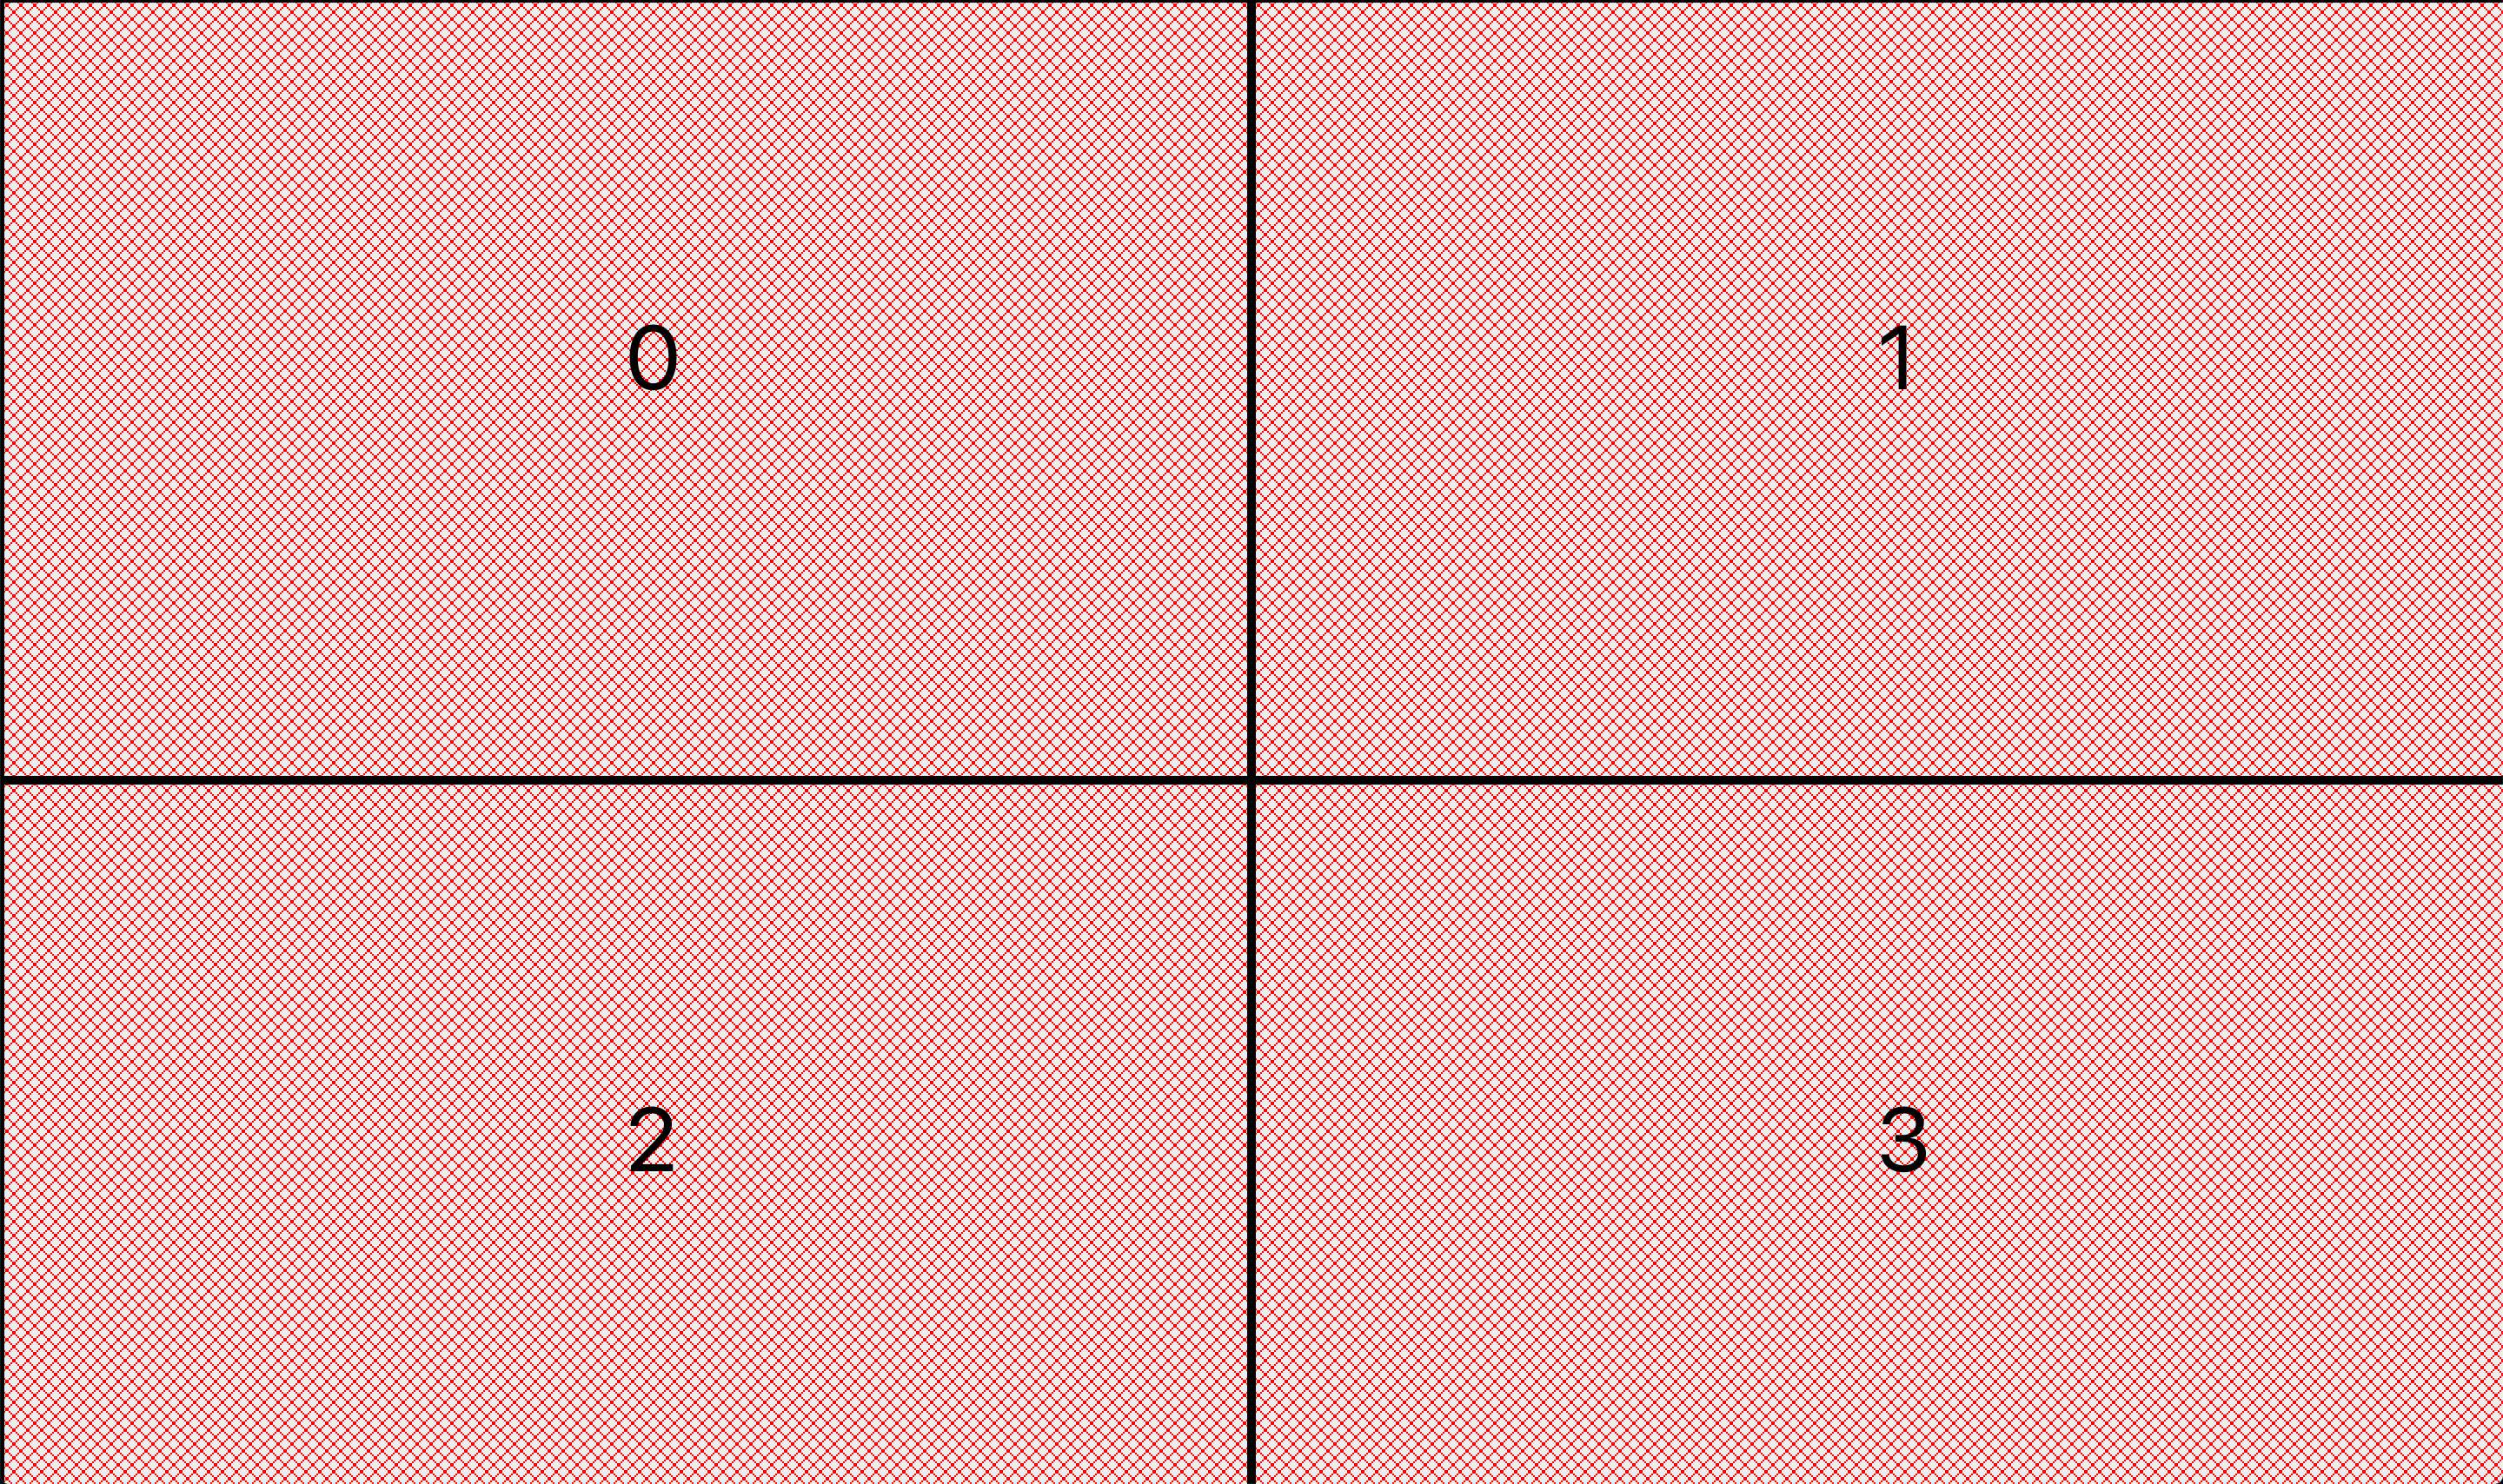
\includegraphics[width=\textwidth/3 - 5pt]{grid_2_2.png}
    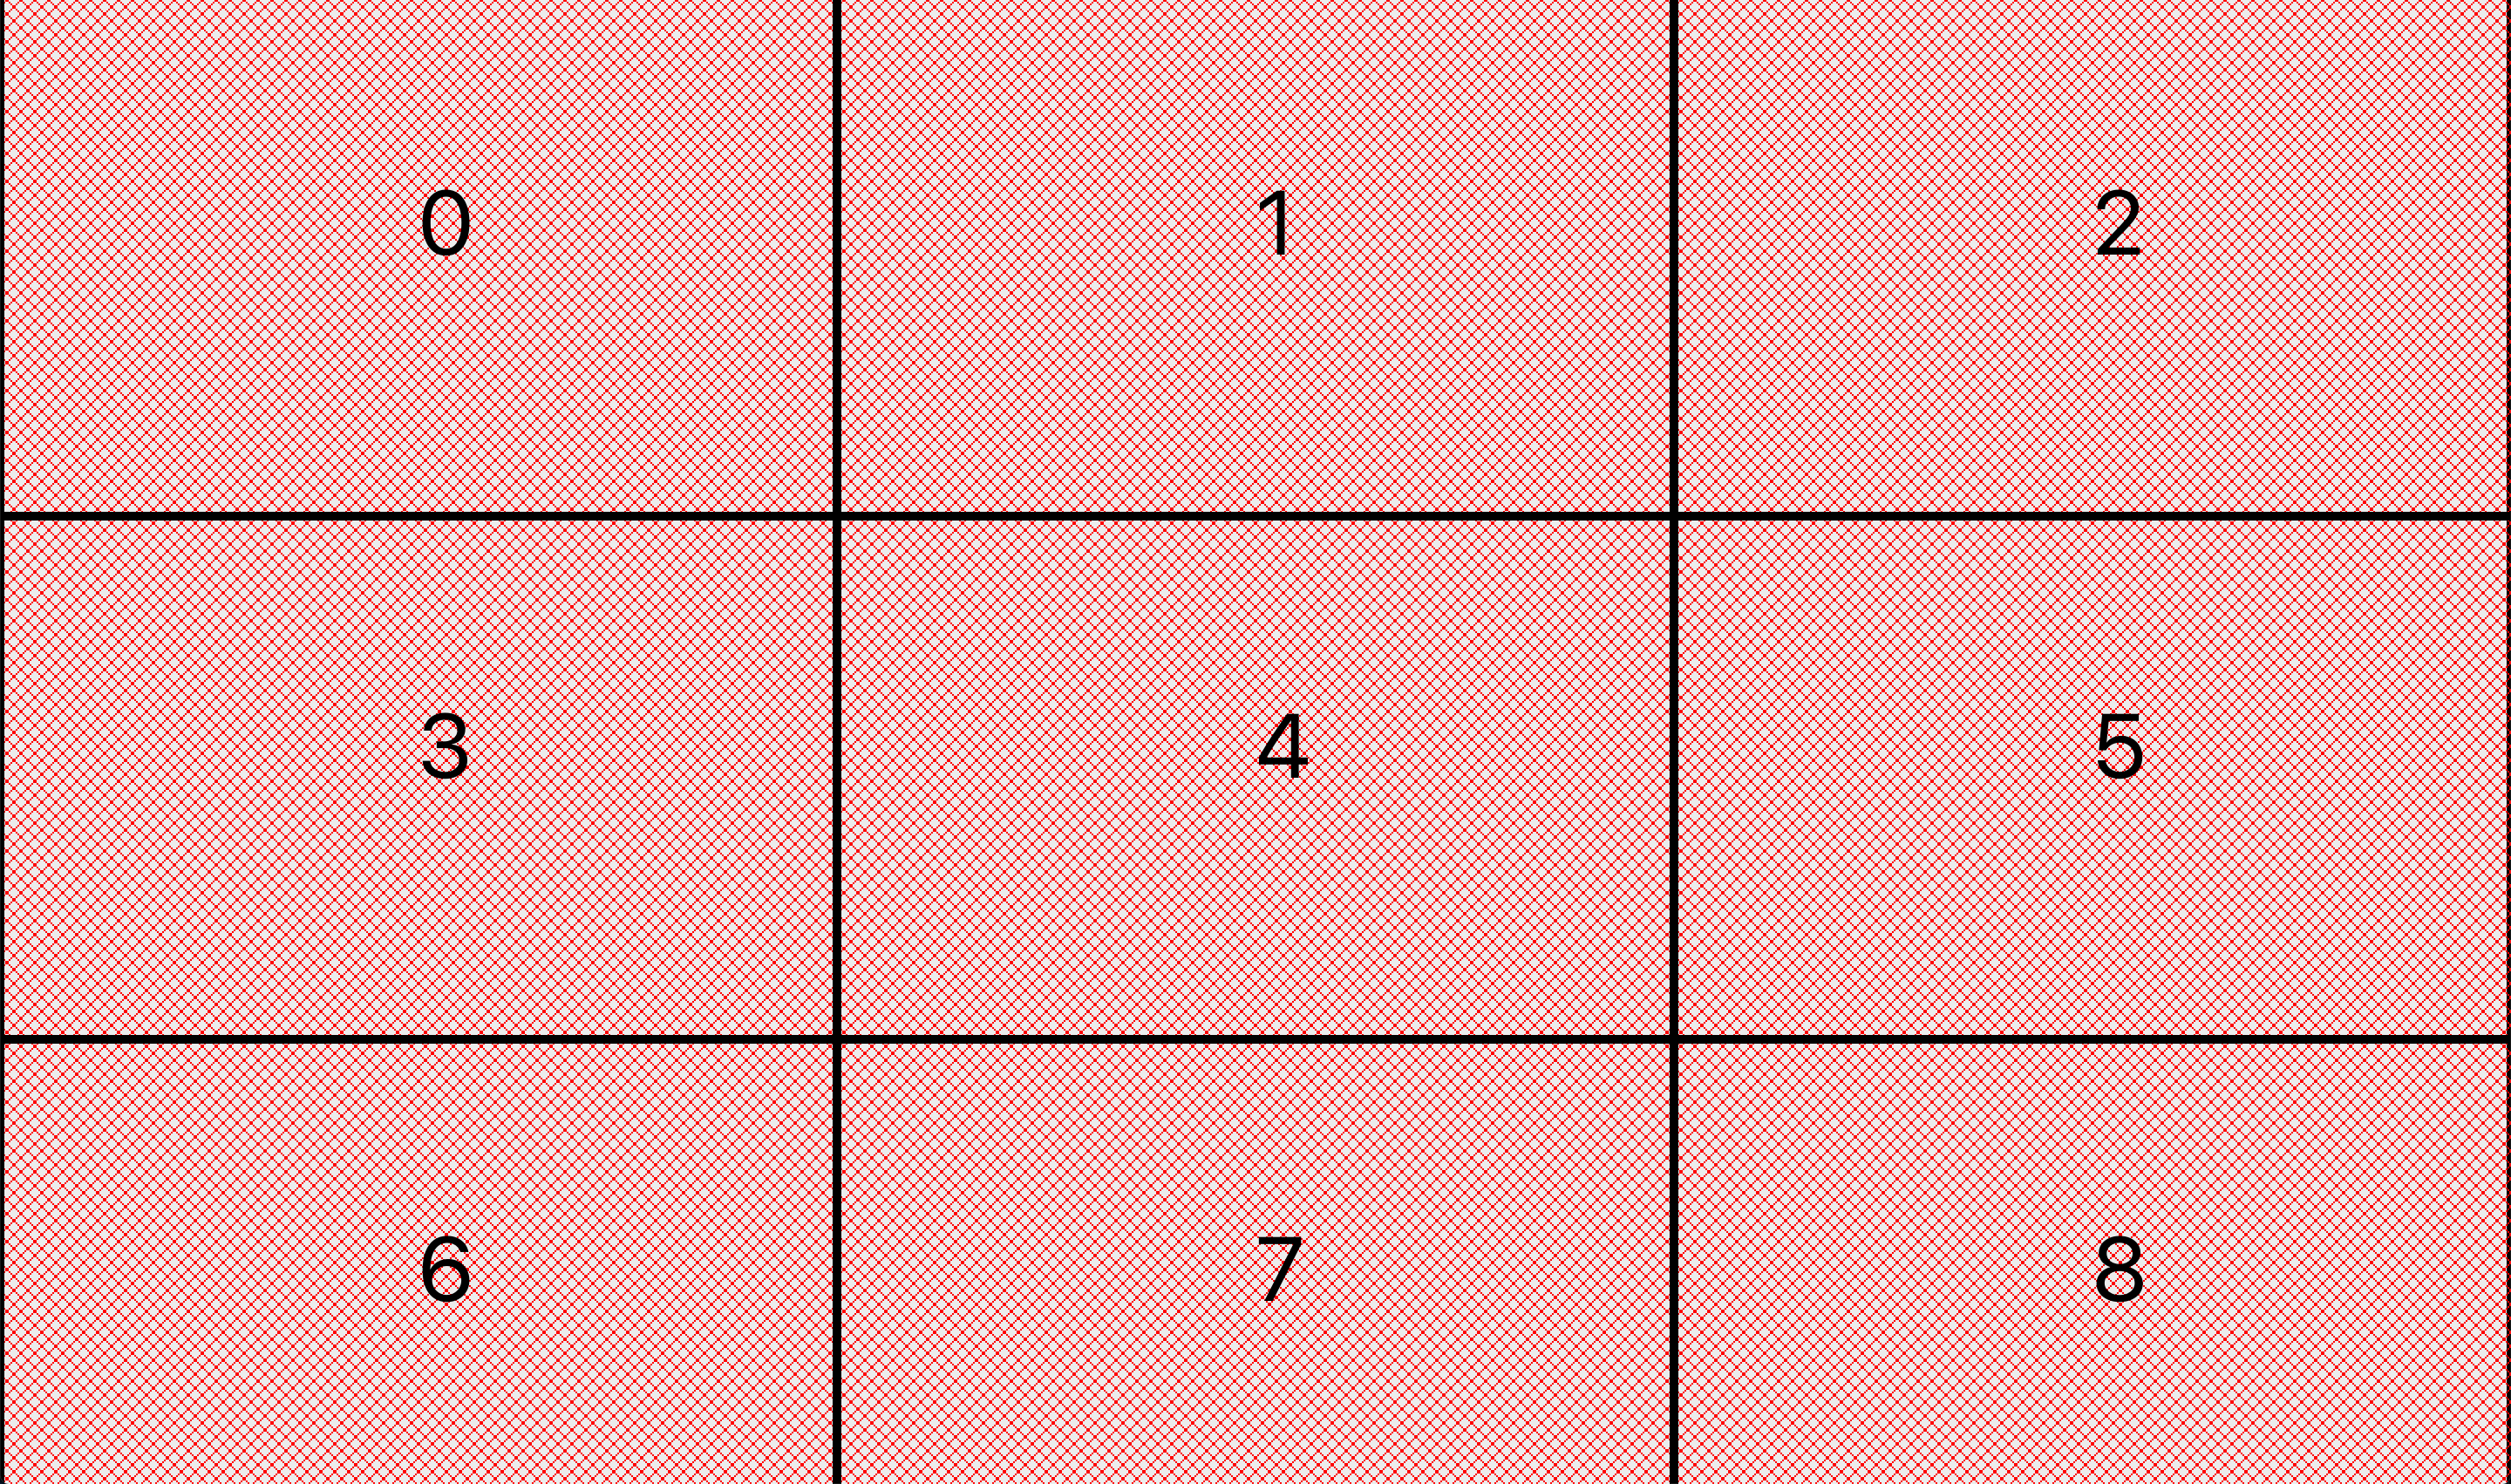
\includegraphics[width=\textwidth/3 - 5pt]{grid_3_3.png}
    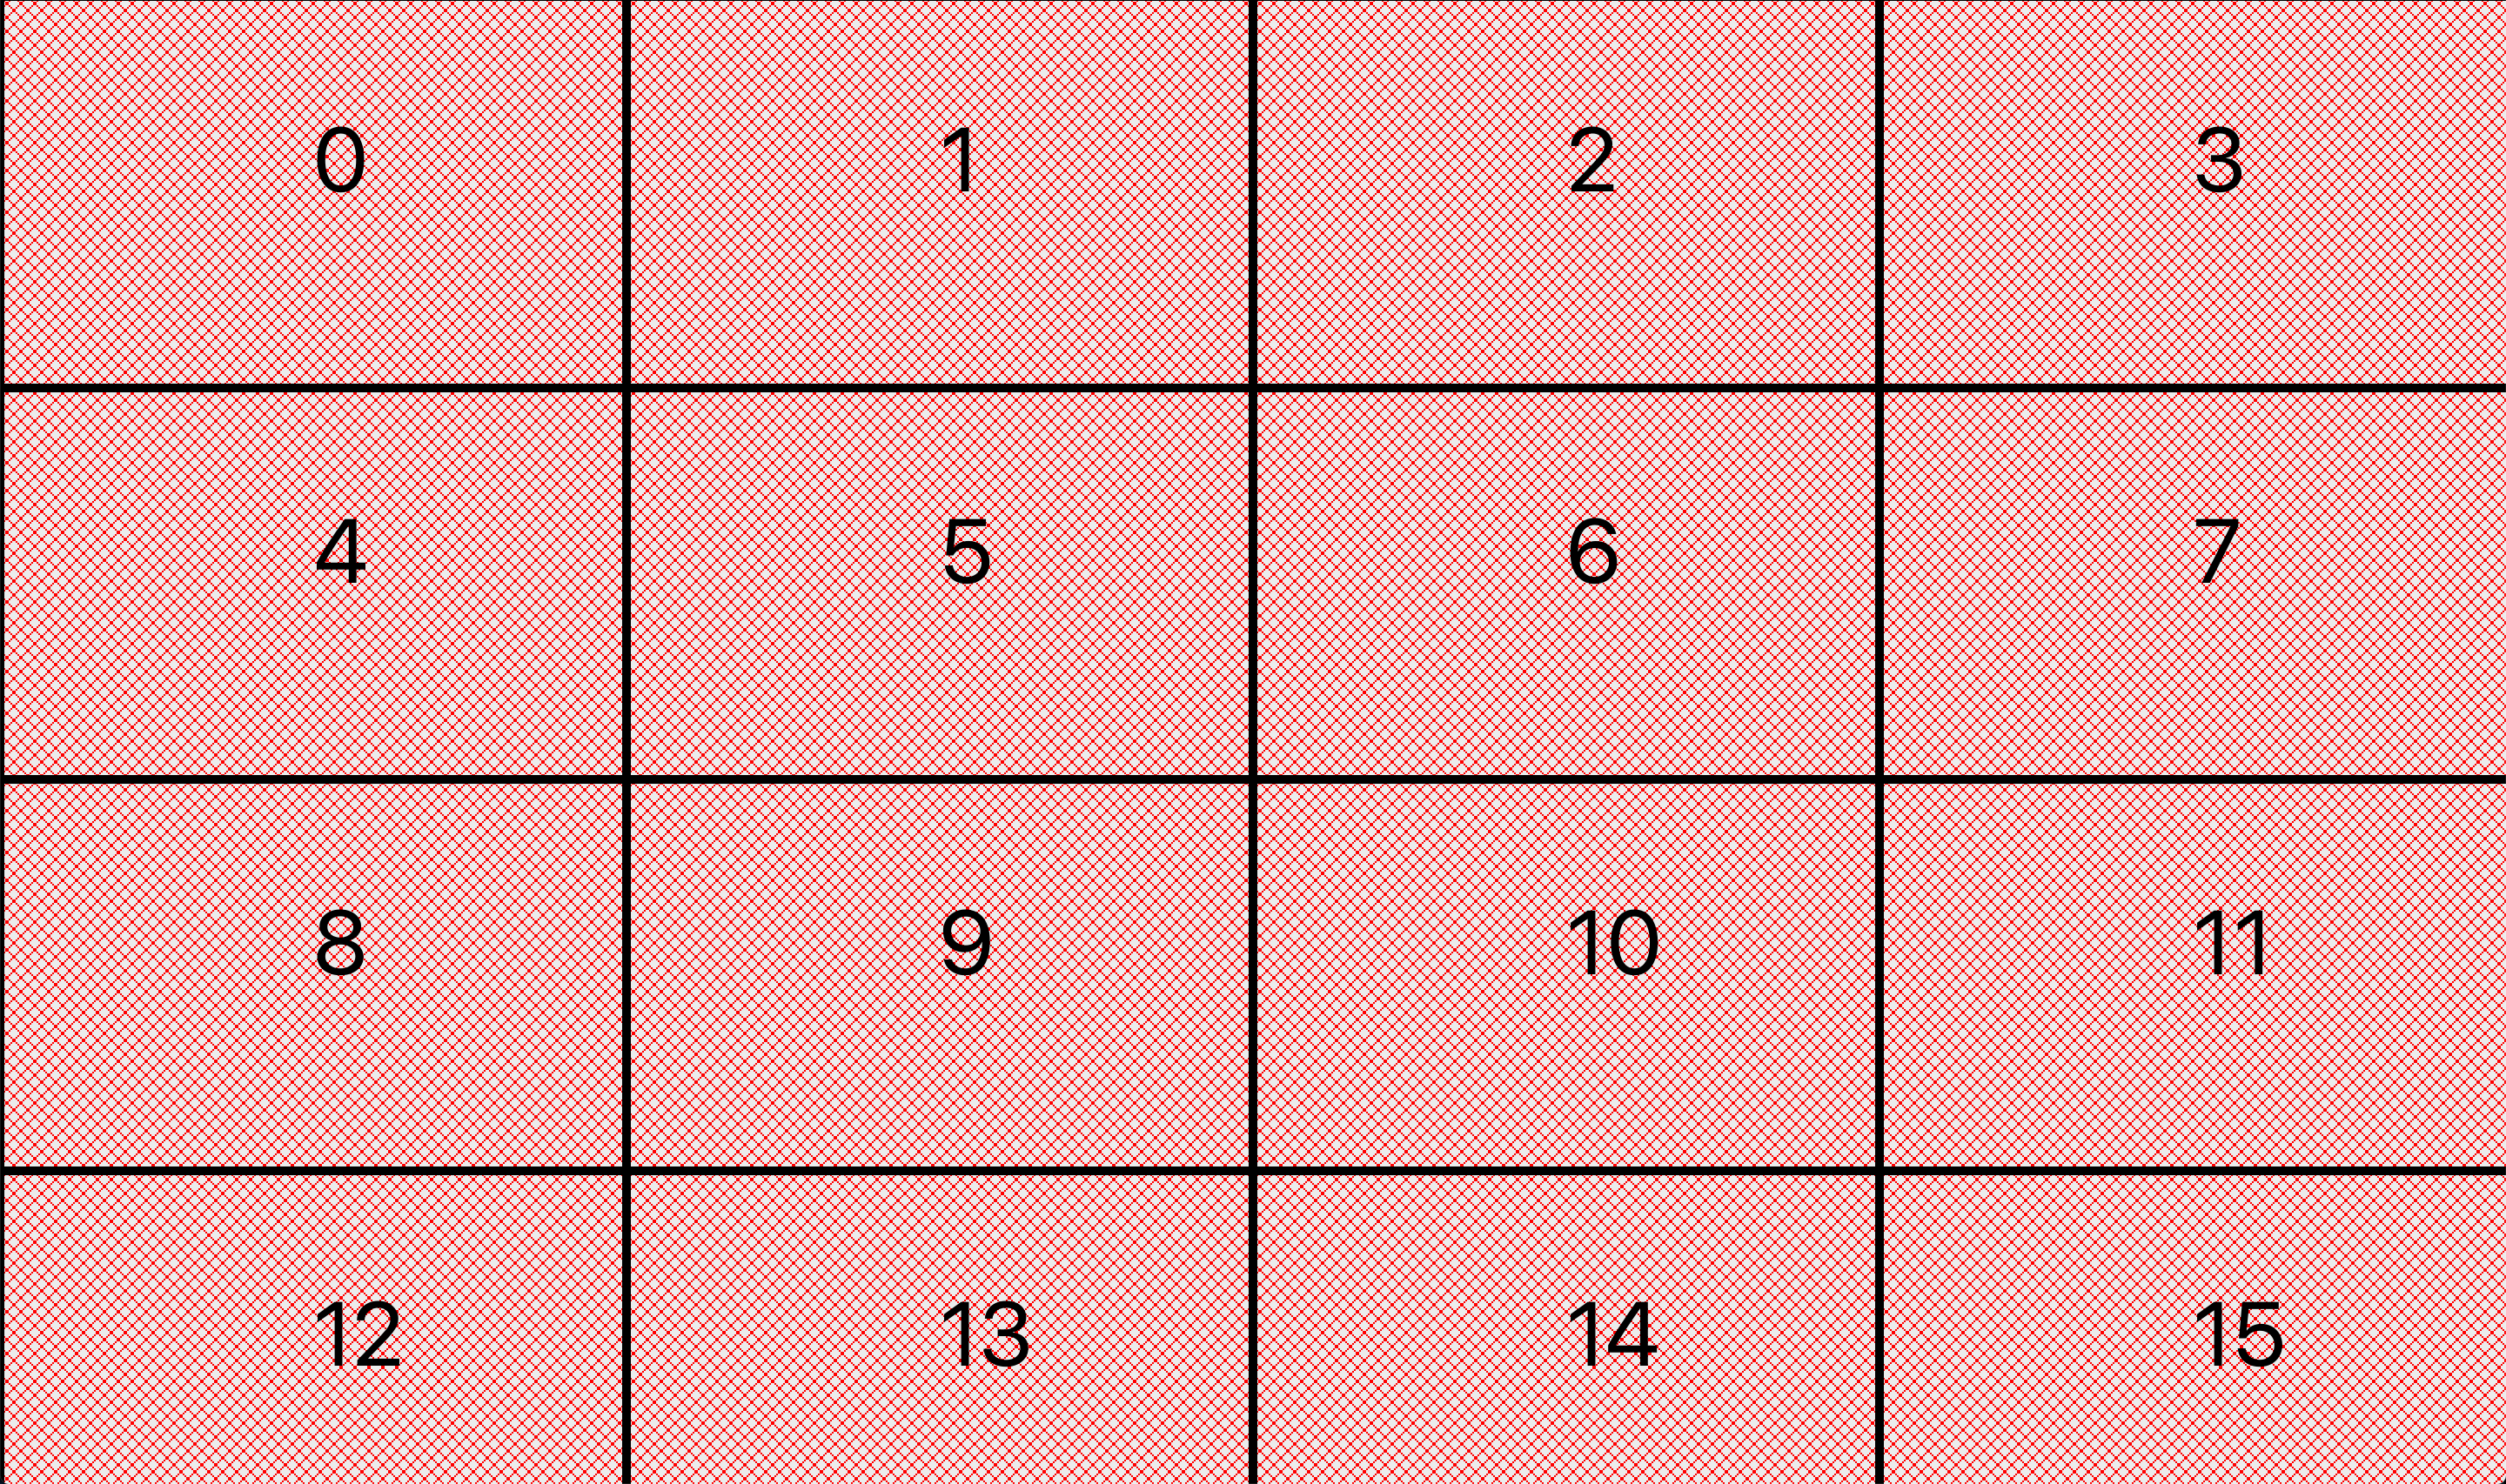
\includegraphics[width=\textwidth/3 - 5pt]{grid_4_4.png}
    \caption{Exemples de grilles}
    \label{grid-example}
\end{figure}

\paragraph{}
Deuxièmement, je vais essayer de simuler les fonctions de clic comme suit: si l'utilisateur ferme son œil gauche pendant un certain temps, nous interpréterons cela comme un clic gauche.
La même chose sera faite pour le clic droit, en utilisant l'œil droit.
% Secondly, I will try to simulate the click functions as follows: if the user closes his left eye for a certain amount of time, then we will interpret that as a left click.
% The same will be done for the right click, using the right eye.

\paragraph{}
A titre d'orientation générale, je vais essayer de développer l'application afin qu'elle soit facilement maintenable.
Je me concentrerai également sur les concepts que j'ai appris tout au long de mes études universitaires: ``clean code'', principes OOP, principes SOLID, cohésion, etc.
Une bonne condition serait également de rendre l'application multiplateforme.
% As some general guidelines, I will try to develop the application in order for it to be easily maintanable.
% I'll also focus on concepts I have learned throughout university: clean code, OOP principles, SOLID principles, cohesion etc.
% Also, a good requirement would be to make the application cross-platform.

\subsection{Objectifs préférables}
\paragraph{}
Pour aller un peu plus loin, si la prédiction des carrés se passe bien, on peut essayer de prédire l'emplacement exact du curseur.
Cela signifie que nous déplacerons le curseur de la souris exactement là où nous pensons que l'utilisateur regardera.
% To go a little further, if predicting the squares goes well, we can try to predict the exact location of the cursor.
% That means we'll move the mouse cursor exactly where we think the user will be looking.

\paragraph{}
Avoir plus d'informations sur l'utilisateur pourrait nous aider dans nos calculs.
Pour cela, je vais aussi essayer de voir comment je peux utiliser d'autres parties du visage pour améliorer les calculs: par exemple, la position du nez.
L'image ci-dessous représente quelques points de repère du visage que nous utiliserons pour nos calculs: les points $[37, 48]$ sont pour les yeux et $[28, 36]$ pour le nez.
% Having more information about the user could help our calculations.
% For that, I will also try to look into how I can use other parts of the face to improve the calculations: for example, the nose position.
% The image below represents some facial landmarks we will use for our calculations: points $[37, 48]$ are for eyes and $[28, 36]$ for the nose.
\begin{figure}[H]
    \centering
    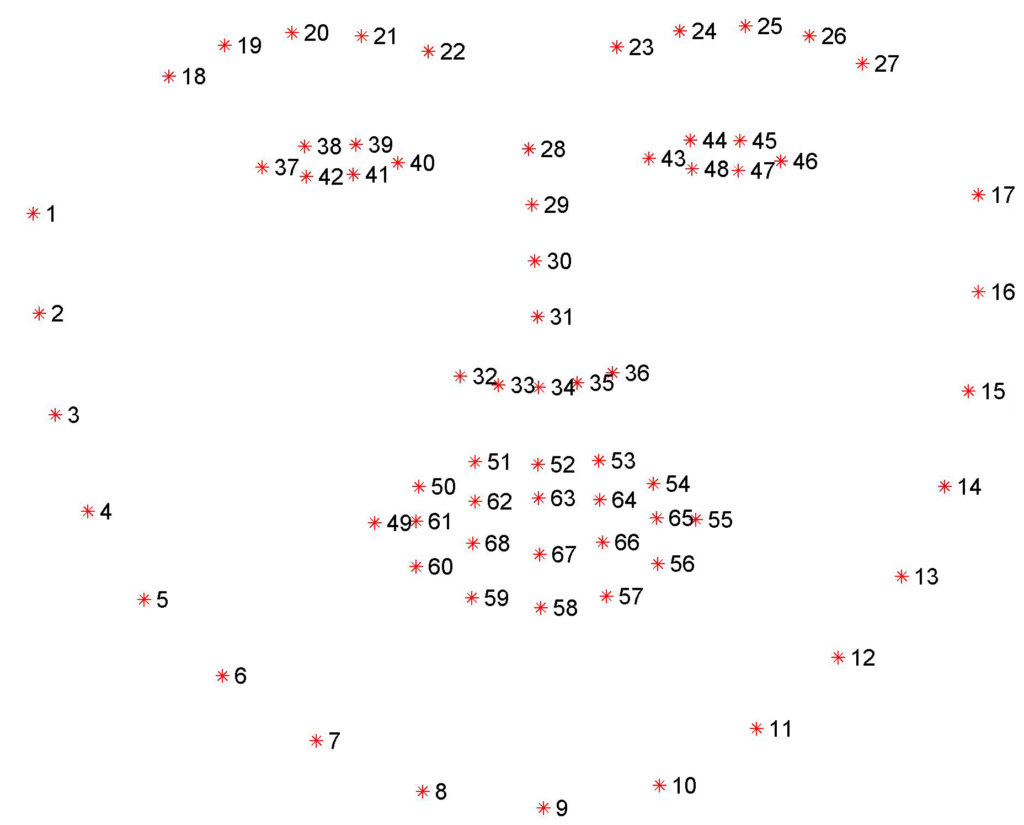
\includegraphics[width=\textwidth/2 - 10pt]{facial_landmarks_1.jpg}
    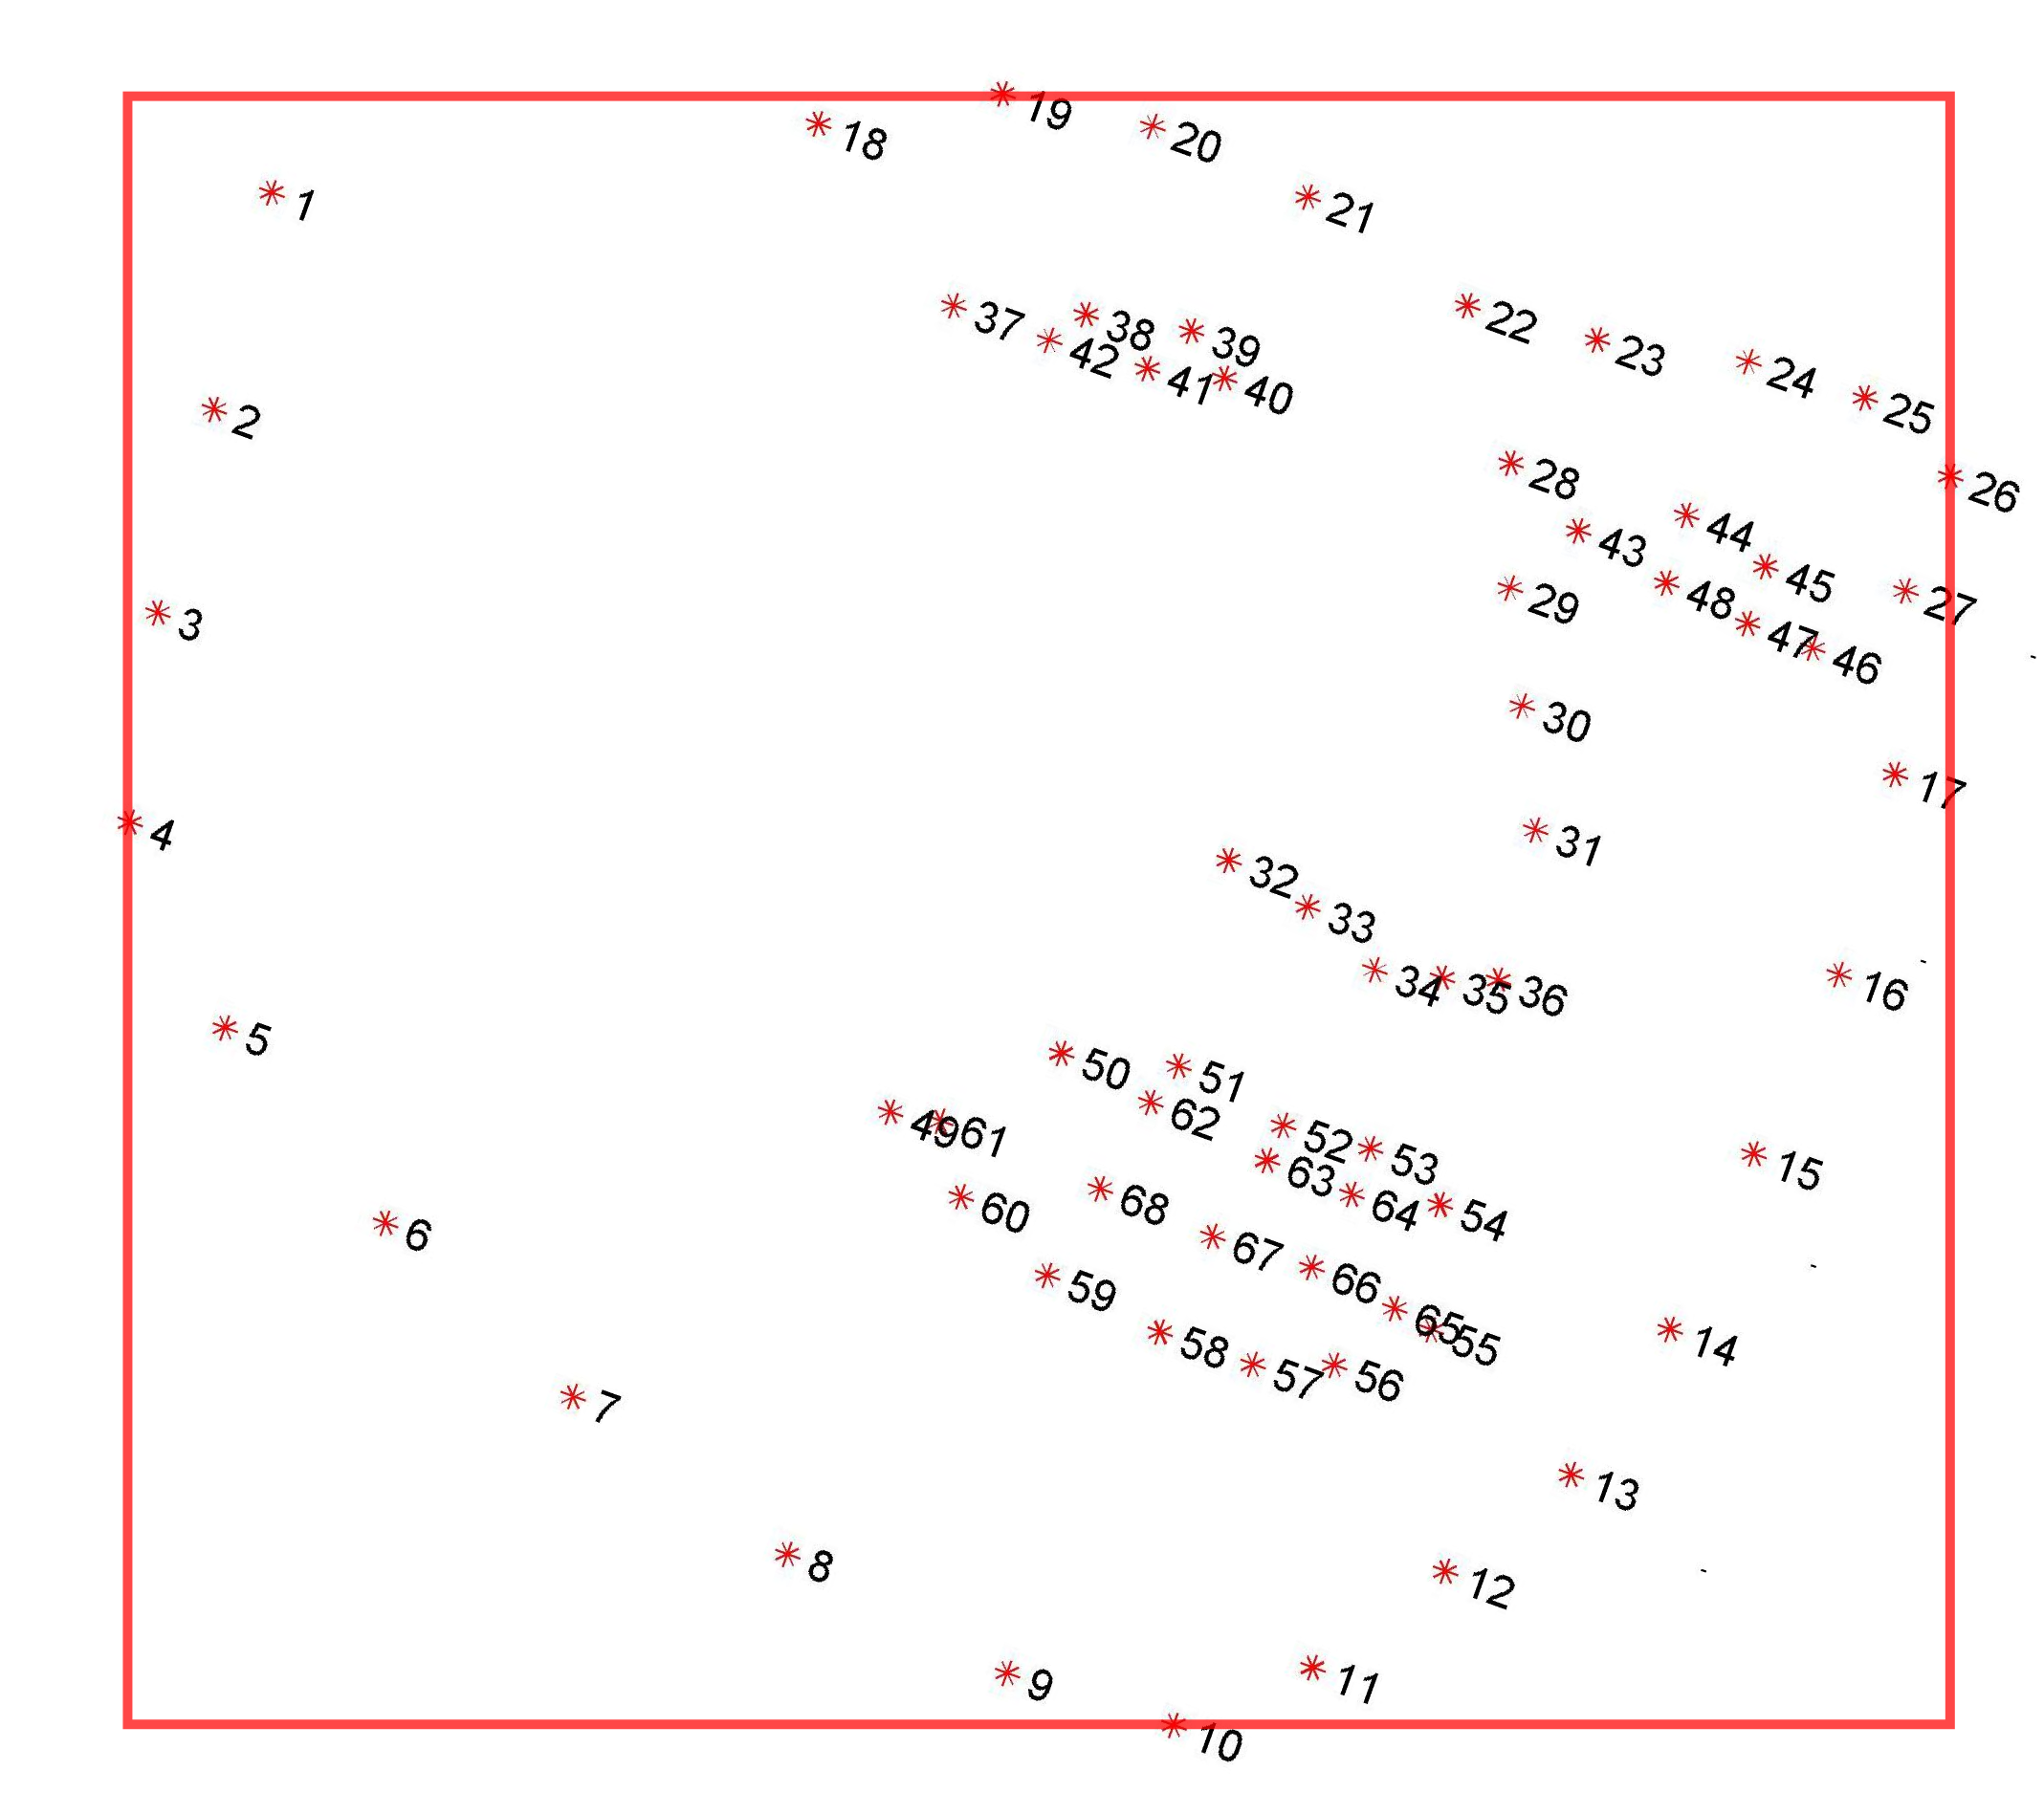
\includegraphics[width=\textwidth/2 - 10pt]{facial_landmarks_2.png}
    \caption{Repères faciaux\\Source: \href{https://ibug.doc.ic.ac.uk/resources/300-W/}{ibug}}
    \label{figure:facial-landmarks}
\end{figure}